\documentclass[a4paper]{article}

%% Language and font encodings
\usepackage[german]{babel}
\usepackage[utf8x]{inputenc}
\usepackage[T1]{fontenc}
\usepackage{float}

%% Sets page size and margins
\usepackage[a4paper,top=3cm,bottom=2cm,left=3cm,right=3cm,marginparwidth=1.75cm]{geometry}

%% Useful packages
\usepackage{amsmath}
\usepackage{graphicx}
\usepackage[colorinlistoftodos]{todonotes}
\usepackage[colorlinks=true, allcolors=blue]{hyperref}
\usepackage{chngcntr}
\usepackage{color}
\usepackage{wrapfig}
\usepackage{pdfpages}
\usepackage{longtable}

  
%% Definitions
\newcommand{\entspricht}{\mathrel{\widehat{=}}}
\counterwithin*{equation}{section}
\counterwithin*{equation}{subsection}
\counterwithin*{equation}{paragraph}


\title{Open CheatSheet: GdI-Edition}
\author{Source \url{https://github.com/hubwoop/ocs-gdi-ohm}}

\begin{document}
\maketitle

\section{Tabellenwerk}
	\begin{table}[H]
	\centering
	\caption{Umrechnung zu dezimal bis $b^{12}$}
	\label{gaengigeWerte}
	\begin{tabular}{l|c|c|c|c|c|c|c|c|c|c|c|c|c}
	         & $b^{0}$&$b^{1}$&$b^{2}$&$b^{3}$&$b^{4}$&$b^{5}$&$b^{6}$&$b^{7}$&$b^{8}$&$b^{9}$&$b^{10}$&$b^{11}$&$b^{12}$ \\ \hline\hline
	$b = 2$  & 1      & 2     & 4     & 8     & 16    & 32    & 64    & 128   & 256   & 512   & 1024   & 2048   & 4096    \\
	$b = 8$  & 1      & 8     & 64    & 512   & 4096  & -     & -     & -     & -     & -     & -      & -      & -       \\
	$b = 16$ & 1      & 16    & 256   & 4096  & 65536 & -     & -     & -     & -     & -     & -      & -      & -       \\
	\end{tabular}
	\end{table}

	\begin{table}[H]
	\centering
	\caption{Gängige Zahlensysteme: Darstellungen bis Wert 15}
	\label{hexWerte}
	\begin{tabular}{l|c|c|c|c|c|c|c|c|c|c|c|c|c|c|c|c}
	$dez$ & 0 & 1 & 2  & 3  & 4   & 5   & 6     & 7     & 8    & 9    & 10   & 11   & 12   & 13   & 14   & 15   \\ \hline\hline
	$bin$ & 0 & 1 & 10 & 11 & 100 & 101 & 110   & 111   & 1000 & 1001 & 1010 & 1011 & 1100 & 1101 & 1110 & 1111 \\
	$oct$ & 0 & 1 & 2  & 3  & 4   & 5   & 6     & 7     & 10   & 11   & 12   & 13   & 14   & 15   & 16   & 17   \\
	$hex$ & 0 & 1 & 2  & 3  & 4   & 5   & 6     & 7     & 8    & 9    & A    & B    & C    & D    & E    & F    \\
	\end{tabular}
	\end{table}

	\begin{table}[H]
	\centering
	\caption{vielfache von $10_{10}$ (Nützlich für die Berechnung von Dezimalzahlen im Quellsystem)}
	\label{vielfacheVon10}
	\begin{tabular}{cc|c|c|c|c|c|c|c|c}
	Basis &10    & 2    & 3   & 4   & 5   & 6   & 7   & 8   & 9  \\\hline
	      &10    & 1010 & 101 & 22  & 20  & 14  & 13  & 12  & 11 \\\hline
	      &20    &      & 202 & 110 & 40  & 32  & 26  & 24  & 22 \\\hline
	      &30    &      &     & 132 & 110 & 50  & 42  & 36  & 33 \\\hline
	      &40    &      &     &     & 130 & 104 & 55  & 50  & 44 \\\hline
	      &50    &      &     &     &     & 122 & 101 & 62  & 55 \\\hline
	      &60    &      &     &     &     &     & 114 & 74  & 66 \\\hline
	      &70    &      &     &     &     &     &     & 106 & 77 \\\hline
	      &80    &      &     &     &     &     &     &     & 88
	\end{tabular}
	\end{table}

\section{Rechnen in b-Adischen Systemen}
	\subsection{Subtraktion}
		Beispiel: $(11)_4 - (2)_4 = (2)_4$\\Wie geht das: Man leiht sich eine 1 von der nächsten stelle und hat somit effektiv $(4+1-2)_{10} = 3_{10} = 3_{4}$
\section{Umrechnen}
	\subsection{\texorpdfstring{$b = 10$ zu $b \neq 10$ (Basis 10 zu beliebige Basis ungleich 10)}{Basis 10 zu b-adisch ungleich 10}}
		\begin{enumerate}
			\item Rechne mod b notiere Rest als letzte stelle des Ergebnisses
			\item Rechne mod b von Ganzahlanteil von Schritt notiere Stelle als vorletzte des Ergebnisses
			\item Setze fort bis Ganzahlanteil = 0
		\end{enumerate}
	\subsection{\texorpdfstring{$b \neq 10$ zu $b = 10$ (beliebige Basis ungleich 10 zu Basis 10)}{b-adisch ungleich 10 zu Basis 10}}
		\subsubsection{Im Zielsystem}
			Stellen addieren nach folgender Vorschrift:
			\[
			 \sum \limits_{n=0}^{N-1} (a_n * b^{n}), a_n \in \{0, \ldots , b-1\}, i \in \{0, \ldots ,N-1\}
			\]
			wobei $N$: Anzahl der Stellen, $n$: Stelle der Zahl und $a_n$: Wert der Ziffer an Stelle $n$.
			
		\subsubsection{\texorpdfstring{Ein Beispiel: $(124032)_5$}{Ein Beispiel: Basis 5}}
			\[
			(124032)_5 = (1*5^{5})+(2*5^{4})+(4*5^{3})+(0*5^{2})+(3*5^{1})+(2*5^{0}) = 3125 + 1250 + 500 + 0 + 15 + 2 = 4892
			\]
	
	\subsection{\texorpdfstring{Im Quellsystem}{Rechnen im Quellsystem: Von b-adisch ungleich 10 zu Basis 10}}
	Rechnen im Quellsystem zur Umwandlung von Zahlen beliebiger b-adischer Systeme zum dezimal System
	
		\subsubsection{Der Algorithmus in Worten}
			\begin{enumerate}
			\item Teile die umzurechnende Zahl durch die Repräsentation der $(10)_{10}$ im Quellsystem bis das Ergebnis der Subtraktionen (innerhalb des Divisionsalgorithmus) nicht mehr durch "10" teilbar sind. Das letzte Ergebnis der Subtraktion ist der Divisionsrest.
			\item Wiederhole Schritt 1 für jedes Ergebnis (ohne Rest) bis das Resultat nur noch einen Rest Darstellt. (Das heißt Ganzzahlanteil = 0)
			\item Die Reste der Divisionen sind die Quellsystemrepräsentanten der einzelnen Stellen der zu berechnenden Dezimalzahl. Die hochwertigste Stelle entspricht der zuletzt vorgenommenen Division.
			\end{enumerate}
	
		\subsubsection{\texorpdfstring{Ein Beispiel: $(120102)_3$ zu $(416)_{10}$}{Ein Beispiel: 120102 Basis 3 zu Dezimal 416}}
			Folgende Tabelle hilft bei der Berechnung der Divisionen. Man braucht nur vielfache bis $b-1$ zum berechnen der Divisionen.
			\begin{table}[H]
			\centering
			\caption{Vielfache von $(10)_{10}$ im 3-er System}
			\label{vielfacheVon10in3}
			\begin{tabular}{c|c}
			Basis 10 & basis 3 \\\hline
			10       & 101     \\\hline
			20       & 202
			\end{tabular}
			\end{table}
			\begin{eqnarray}
			120102 / 101 =  1112\;R\:20 \\
			1112 / 101 = 11\;R\:1 \\
			11 / 101 = 0\;R\:11
			\end{eqnarray}
			Aus (3) $ \Rightarrow  (11)_3 \entspricht (4)_{10} $ \\
			Aus (2) $ \Rightarrow  (1)_3 \entspricht (1)_{10} $ \\
			Aus (1) $ \Rightarrow  (20)_3 \entspricht (6)_{10} $ \\
			
			$ \Rightarrow (416)_{10} $

\section{Vorzeichenbehaftete Darstellungen}
	\subsection{Komplementbildung}
			$(b-1) - Stelle$ bedeutet für bspw. für hex $15-$stelle
		\paragraph{Beispiel Oktalsystem}
			Komplement von $00354 = 77423$ weil $b-1 = 7$ und somit lautet die Berechnung für jede stelle v.l.n.r: $7-0=7, 7-0=7,7-3=4,7-5=2,7-4=3 \rightarrow 77423$
	\subsection{kleinste / größte darstellbare Zahl mit N Bits}
		\paragraph{Exzess-N}
		kleinste: -N; Größte: N-1\\
		größte positive: $2^{Anzahl~der~bits}$ - 1 - Exzesswert\\
		kleinste negative: -Exzesswert
		\paragraph{b-1-Komplement}
		$[ -(2^{N-1}-1) … +(2^{N-1}-1)]$\\
		doppelte null: 0000 und 1111 sind beides null
		\paragraph{b-Komplement}
		$[ - 2^{N-1} … +2^{N-1} - 1]$
		
	\subsection{Rechnen mit dem einer Komplement}
		Den einer Rücklauf beachten (carry bit von höchster stelle wird (falls vorhanden) zum Ergebnis addiert (Ergebnis + 1)
	\subsection{Rechnen mit dem zweier Komplement}
		nach der Komplementbildung eins addieren.
	\subsection{Exzesscode}
		Sinnvollste Darstellung $2^{Anzahl der Bits} / 2$\\
		Umwandlung zu Exzess ist immer: darzustellende Zahl + Exzesszahl ($2^{Anzahl der Bits} / 2$)
		Unwandlung von Exzess ist immer: Codierte Zahl - Exzesszahl
		
	\subsection{Welche Zahlen sind im b-Komplement negativ}
		\paragraph{bei geraden basen} ist die erste Ziffer größergleich $ b / 2 $ gilt die zahl als negativ ansonsten ist sie positiv \\
		So sind die vorzeichenlosen Zahlen $1 … (b^N/2)-1$ im b-Komplement positiv, $(b^N/2) … b^N-1$ sind negativ, $0$ ist null.\\
		Im (b-1)-Komplement gilt, dass die Zahlen $(b^N/2) … b^N-2$ negativ sind, $b^N-1$ ist minus null.
		\paragraph{bei ungeraden basen}
		Hier wird die Trennlinie bei der Zahl $(aaa...a)_b$ gezogen, wobei $a=(b-1)/2$ ist. Bei$ b=3$ ist es die Zahl $(111...1)_3$.
	
\section{Reele Zahlen}
	\subsection{2-adische Entwicklung (Dezimal zu Binär wandeln)}
		\begin{enumerate} 
			\item Multipliziere die Dezimalzahl mit 2
			\item Wenn Ergebnis < 0 notiere null ansonsten notiere 1 und ziehe 1 vom Ergebnis eins ab
			\item wiederhole Schritt 1 mit Ergebnis der bisherigen Schritte
			\item Erstes Ergebnis: Erste Stelle nach dem Komma 
		\end{enumerate}
		Trick: Wenn die Zahl welche binär dargestellt werden soll eine Zweierpotenz im Nenner hat, dann stellt der Wert des Exponenten die Anzahl der Nachkommastellen dar. Also bspw. $ 1/8 = 1/2^3 $ dar. Daraus folgt 3 Nachkommastellen (weil der Exponent die drei ist). Die Zahl auf dem Bruch wird dann von rechts eingeschoben also bspw. $2/8 = 2/2^3 $ => drei Nachkommastellen und $ 2 = 01 $ daraus folgt das Ergebnis: $ 0.010 = 1/4$
		\paragraph{Beispiel} Umwandlung Dezimal zu Binär $(0.2)_{10}$\\
			$0.2 * 2 = 0,4 $ Notiere 0\\
			$0.4 * 2 = 0,8 $ Notiere 0\\
			$0.8 * 2 = 1,6 $ Notiere 1 und ziehe eins von $1,6 ab$\\
			$0.6 * 2 = 1,2 $ Notiere 1 und ziehe eins von $1,2 ab$\\
			$0.2 * 2 = 0,4 $ Periodische Dualzahl entdeckt\\
			$(0.2)_{10} = 0.\overline{0011}$
		
		
	\subsection{Konvertieren zwischen Binär/Hexadezimal/Dezimal}
		Folgende Beispiele beschreiben das Schema:
		
		\paragraph{Vorkomma Anteil} 
			(siehe Kapitel 2 und 3 - Umrechnen ganzer Zahlen)
			\begin{eqnarray}
			10110.110010 \\
			0001 = (1)_{16} \\
			0110 = (6)_{16}\\
			\Rightarrow (16)_{16} \\
			(16)_{16} = (22)_{10}
			\end{eqnarray}
		
		\paragraph{Nachkomma Anteil zu dez}
			Aufsummieren:
			$N*b^{-1}+N*b^{-2}+...+N*b^{-i} $ wobei i die letzte Nachkommastelle ist und N der wert der stelle
		
		\paragraph{Shortcut bei Zahlen mit nur einsen nach dem komma}
			Wert von $0.1111$ (also vier stellen nach dem Komma): $(1-2^{-4}) = 2^{-1}+2^{-2}+2^{-3}+2^{-4} = \frac{15}{16}$
		
		\paragraph{Nachkommaanteil von bin zu hex}:\\
			Vierergrüppchen bilden: $ \Rightarrow (10110.110010)_{2} = (0001)(0110).(1100)(1000) = (16.C8)_{16}$ 
		
	\subsection{Gleitkommazahlen}
		\paragraph{normalisiert} 
			ist eine Gleitkommazahl wenn die Ziffern nach dem Komma sich nicht mehr weiter nach links verschieben lassen ohne das werte über das Komma "hinausrutschen". Die folgenden Werte sind bereits normalisiert:
			\begin{eqnarray}
				0.11001*2^{-39} \\
				0.001011*8^4
			\end{eqnarray}
		\paragraph{normalisieren} 
			Bei positiven Exponenten gilt: wenn die zahlen nach links geschoben werden müssen muss vom Exponenten abgezogen werden, wenn die zahlen nach rechts geschoben werden muss man zum Exponenten addieren.\\
			Bei negativen verhält es sich genau anders herum.\\
			$0.001011 \cdot 2^{12} = 0.1011 \cdot 2^{10}$\\
			Dabei unbedingt auf die Exponentenbasis achten! Im Dualsystem zur Basis zwei normalisieren geht einfach: pro geschobene stelle wird der Exponent um eins erhöht/erniedrigt. Bei Exponentenbasis 8 kann nur um 3 stellen geschoben werden(pro Exponentveränderung um 1), weil $8 = 2^3$!\\
			$0.00011001 \cdot 8^{-12} = 0.11001 \cdot 8^{-13}$
		\paragraph{Unterlauf- und Überlaufbereich}
			Unterlauf: Kleinste zulässige(!) Darstellung wählen und Dezimalwert berechnen. Dabei darauf achten: wenn Normalisierung gefordert wird, ist die kleinste zulässige Mantisse nicht 0.000001 sonder 0.1. In IEEE ist bspw. keine Normalisierung gefordert, daher kann man hier wirklich den kleinst möglichen Mantissenwert annehmen.
		\paragraph{Floating-Point generell: Abstand zwischen zwei Ziffern in einem Bereich} (Auflösung bestimmen)
			\\Wähle die größere Zahl (von den Rändern des zu untersuchenden Bereiches) und multipliziere diese mit dem niedrigsten Mantissenbit $(2^{-laenge~der~Mantisse}) \cdot groessere~rand~zahl$.\\
			\\Beispiele für eine Darstellung mit 15-Bit-Mantisse:
			\\Bereich: $2^{-15} \leq z < 2^{-14}$
			\\Abstand: $(0.000000000000001)_2 \cdot 2^{-14} = 2^{-15}*2^{-14} = 2^{-29}$\\
			\\Bereich: $2^{21} \leq z < 2^{22}$
			\\Abstand: $(0.000000000000001)_2 \cdot 2^{22} = 2^{-15}*2^{22} = 2^{7}$

	\subsubsection{IEEE-Single-Precision Floating Point}
		Wichtiges zuerst:
		\begin{enumerate} 
			\item normalisiert: Exponent: 0 < EXP < 255 Mantisse: jedes Bitmuster
			\item denormalisiert: Exponent: NUR NULLEN Mantisse: jedes Bitmuster UNGLEICH null
			\item Null: Exponent: 0 Mantisse: 0
			\item unendlich: Exponent: NUR EINSEN Mantisse: 0
			\item NaN: Exponent: NUR EINSEN Mantisse: jedes Bitmuster ungleich null
			\item Denormalisierte Darstellung:  Exponent = -126 und 0 vorm Komma (der Mantisse)
		\end{enumerate}
		\paragraph{Umrechnung IEEE zu Dez} 
			von links: Bit 1: Vorzeichen, Bits 2-9 (8bit): Exponent, Bits 10-32 (23bit): Mantisse.\\
			{\Large $z = \pm1.m_1 ... m_{23}*2^{e_1 ... e_8-127}$ mit VZ $1 \stackrel{\wedge}{=} - $ und $0 \stackrel{\wedge}{=} +$} 
			\\ 
		\paragraph{Umrechnen Dez zu IEEE}
			\begin{enumerate} 
				\item Normalisieren auf 1,...
				\item Potenz zu basis 2 sicherstellen
				\item Mantisse zu dual wandeln
				\item Potenz = potenz + 127
				\item Potenz zu dual wandeln
				\item Erstes Ergebnis: Erste Stelle nach dem Komma 
			\end{enumerate}
		\paragraph{IEEE single precision: Abstand zwischen zwei Ziffern in einem Bereich} (Auflösung bestimmen)
			\\Wähle die kleinere Zahl (von den Rändern des zu untersuchenden Bereiches) und multipliziere diese mit dem niedrigsten Mantissenbit $(2^{-23}) \cdot kleinere~rand~zahl$.\\
			\\Beispiele für IEEE-Single-Precision:
			\\Bereich: $2^{-15} \leq z < 2^{-14}$
			\\Abstand: $(0.00000000000000000000001)_2 \cdot 2^{-15} = 2^{-23}*2^{-15} = 2^{-38}$\\
			\\Bereich: $2^{21} \leq z < 2^{22}$
			\\Abstand: $(0.00000000000000000000001)_2 \cdot 2^{21} = 2^{-23}*2^{21} = 2^{-2}$

\section{Logische Schaltungen}
	\subsection{Symbolik}
		+ = oder\\
		* = und
	\subsection{Minterme und Maxterme}
		\begin{table}[H]
		\centering
		\caption{Minterm/Maxterm Vergleich mit aussicht auf DNF und KNF}
		\label{my-label}
		\begin{tabular}{llllll}
			$x_2$ & $x_1$ & $x_0$ & $a_0$ 	   & Minterm            		  			& Maxterm            							\\
			1    & 1    & 0    & \textbf{0}    &  	&  $\overline{x_2} +  \overline{x_1} +  x_0$	\\
			0    & 1    & 1    & \textbf{1}    &  $\overline{x_2} \cdot x_1 \cdot x_0$	& 
		\end{tabular}
		\end{table}
		Minterme: verundung jener elemente die eins ergeben (0 führt zu verneinung)\\
		Maxterme: veroderung jener elemente die 0 ergeben (1 führt zu verneinung)

		
	\subsection{DNF und KNF}
		DNF vernüpft Minterme mit 'oder' $m_1+m_2$ wobei beispielsweise $m_1 = x_1 \cdot x_2 \cdot x_3$\\
		KNF verknüpft Maxterme mit 'und': $(M_1)\cdot(M_2)$ wobei beispielsweise $M_1 = x_1 + x_2 + x_3$
		
	\subsection{Im KV-Diagram}

		Wenn einsen zusammengefasst werden ergibt sich die DNF\\
		Wenn nullen zusammengefasst werden ergibt sich die KNF\\
		DNF: Variablen am Rand beim zusammenfassen so betrachten wie sie sind\\
		KNF: Variablen am Rand beim zusammenfassen negiert betrachten: Bereiche die NICHT gemeint sind (also ausgeschlossen werden) werden nicht verneint.\\
		Die Maxterm-Methode unterscheidet sich von der Minterm-Methode lediglich in folgenden Punkten:
		\begin{wrapfigure}{r}{0.5\textwidth}
			\vspace{-20pt}
			\begin{center}
				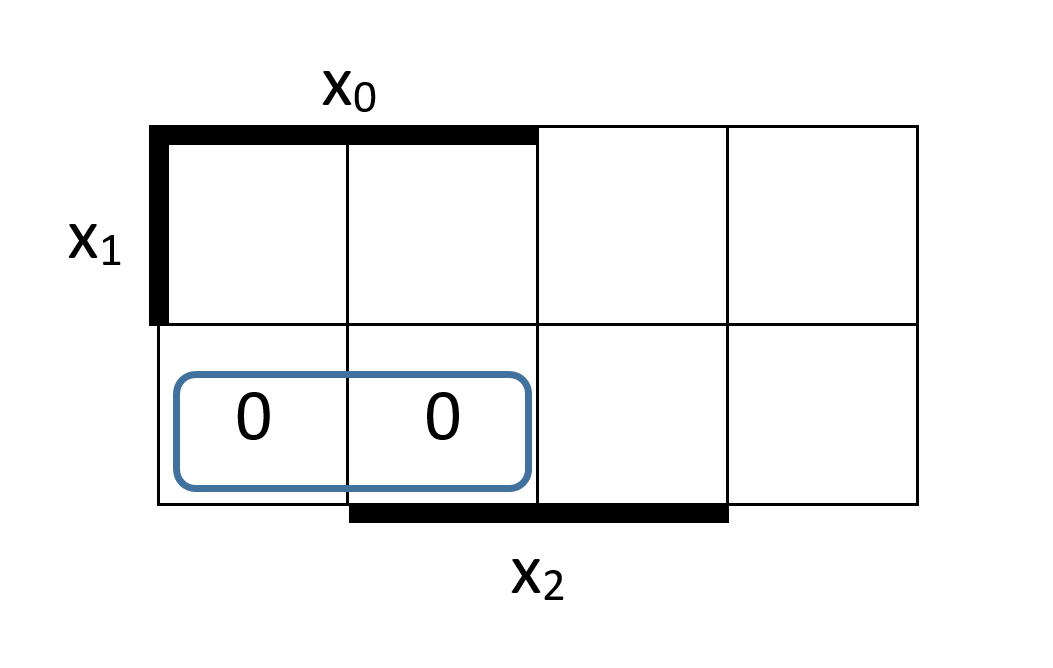
\includegraphics[width=0.48\textwidth]{kv-KNF.png}
			\end{center}
			\vspace{-20pt}
			\caption{KV Diagram KNF lautet: \textcolor{blue}{$\overline{x_0}+x_1$}}
			\vspace{-20pt}
		\end{wrapfigure}

		\begin{enumerate}
			\item Statt Einsen werden Nullen zu Päckchen zusammengefasst.
			\item Ein Päckchen bildet einen Disjunktionsterm (ODER-Verknüpfungen statt eines Konjunktionsterms).
			\item Die Disjunktionsterme werden konjunktiv (mit UND) verknüpft.
			\item Die Variablen werden zusätzlich einzeln negiert.
		\end{enumerate}

\section{Assembler}
	\subsection{Bits zu Assembler wandeln}
		Dabei ist besonders darauf zu achten, dass die Reihenfolge der Bits nicht der Reihenfolge Befehle in Assemblersprache entspricht
	\subsection{Coden}
		Dabei darauf achten, dass oftmals, wenn über Register iteriert wird, auf einen Zähler verzichtet werden kann, da 
		das 'Zielregister' berechnet und als Abbruchbedingung genutzt werden kann.
	\subsection{ASCII-Tabelle}
	
	\begin{figure}[H]
	\begin{longtable}{|c|c|c||c|c|c||c|c|c||c|c|c|}
		\hline
		Dez & Hex  & Zeichen & Dez & Hex  & Zeichen & Dez  & Hex  & Zeichen & Dez & Hex  &  Zeichen   \\
		\hline
		 0  & 0x00 &   NUL   & 32  & 0x20 &   SP    &   64 & 0x40 &    @    & 96  & 0x60 &     `      \\
		 1  & 0x01 &   SOH   & 33  & 0x21 &    !    &	65 & 0x41 &    A    & 97  & 0x61 &     a      \\
		 2  & 0x02 &   STX   & 34  & 0x22 &   "'    &	66 & 0x42 &    B    & 98  & 0x62 &     b      \\
		 3  & 0x03 &   ETX   & 35  & 0x23 &   \#    &	67 & 0x43 &    C    & 99  & 0x63 &     c      \\
		 4  & 0x04 &   EOT   & 36  & 0x24 &   \$    &	68 & 0x44 &    D    & 100 & 0x64 &     d      \\
		 5  & 0x05 &   ENQ   & 37  & 0x25 &   \%    &	69 & 0x45 &    E    & 101 & 0x65 &     e      \\
		 6  & 0x06 &   ACK   & 38  & 0x26 &   \&    &	70 & 0x46 &    F    & 102 & 0x66 &     f      \\
		 7  & 0x07 &   BEL   & 39  & 0x27 &    '    &	71 & 0x47 &    G    & 103 & 0x67 &     g      \\
		 8  & 0x08 &   BS    & 40  & 0x28 &    (    &	72 & 0x48 &    H    & 104 & 0x68 &     h      \\
		 9  & 0x09 &   TAB   & 41  & 0x29 &    )    &	73 & 0x49 &    I    & 105 & 0x69 &     i      \\
		10  & 0x0A &   LF    & 42  & 0x2A &    *    &	74 & 0x4A &    J    & 106 & 0x6A &     j      \\
		11  & 0x0B &   VT    & 43  & 0x2B &    +    &	75 & 0x4B &    K    & 107 & 0x6B &     k      \\
		12  & 0x0C &   FF    & 44  & 0x2C &    ,    &	76 & 0x4C &    L    & 108 & 0x6C &     l      \\
		13  & 0x0D &   CR    & 45  & 0x2D &    -    &	77 & 0x4D &    M    & 109 & 0x6D &     m      \\
		14  & 0x0E &   SO    & 46  & 0x2E &    .    &	78 & 0x4E &    N    & 110 & 0x6E &     n      \\
		15  & 0x0F &   SI    & 47  & 0x2F &    /    &	79 & 0x4F &    O    & 111 & 0x6F &     o      \\
		16  & 0x10 &   DLE   & 48  & 0x30 &    0    &	80 & 0x50 &    P    & 112 & 0x70 &     p      \\
		17  & 0x11 &   DC1   & 49  & 0x31 &    1    &	81 & 0x51 &    Q    & 113 & 0x71 &     q      \\
		18  & 0x12 &   DC2   & 50  & 0x32 &    2    &	82 & 0x52 &    R    & 114 & 0x72 &     r      \\
		19  & 0x13 &   DC3   & 51  & 0x33 &    3    &	83 & 0x53 &    S    & 115 & 0x73 &     s      \\
		20  & 0x14 &   DC4   & 52  & 0x34 &    4    &	84 & 0x54 &    T    & 116 & 0x74 &     t      \\
		21  & 0x15 &   NAK   & 53  & 0x35 &    5    &	85 & 0x55 &    U    & 117 & 0x75 &     u      \\
		22  & 0x16 &   SYN   & 54  & 0x36 &    6    &	86 & 0x56 &    V    & 118 & 0x76 &     v      \\
		23  & 0x17 &   ETB   & 55  & 0x37 &    7    &	87 & 0x57 &    W    & 119 & 0x77 &     w      \\
		24  & 0x18 &   CAN   & 56  & 0x38 &    8    &	88 & 0x58 &    X    & 120 & 0x78 &     x      \\
		25  & 0x19 &   EM    & 57  & 0x39 &    9    &	89 & 0x59 &    Y    & 121 & 0x79 &     y      \\
		26  & 0x1A &   SUB   & 58  & 0x3A &    :    &	90 & 0x5A &    Z    & 122 & 0x7A &     z      \\
		27  & 0x1B &   ESC   & 59  & 0x3B &    ;    &	91 & 0x5B &    [    & 123 & 0x7B &    \{      \\
		28  & 0x1C &   FS    & 60  & 0x3C &   "<    &	92 & 0x5C & $\backslash$ & 124 & 0x7C &       \\
		29  & 0x1D &   GS    & 61  & 0x3D &    =    &	93 & 0x5D &    ]    & 125 & 0x7D &    \}      \\
		30  & 0x1E &   RS    & 62  & 0x3E &   ">    &	94 & 0x5E &  \^{}   & 126 & 0x7E &     "~     \\
		31  & 0x1F &   US    & 63  & 0x3F &    ?    &	95 & 0x5F &   \_    & 127 & 0x7F &    DEL     \\ 
		\hline
	\end{longtable}
\end{figure}

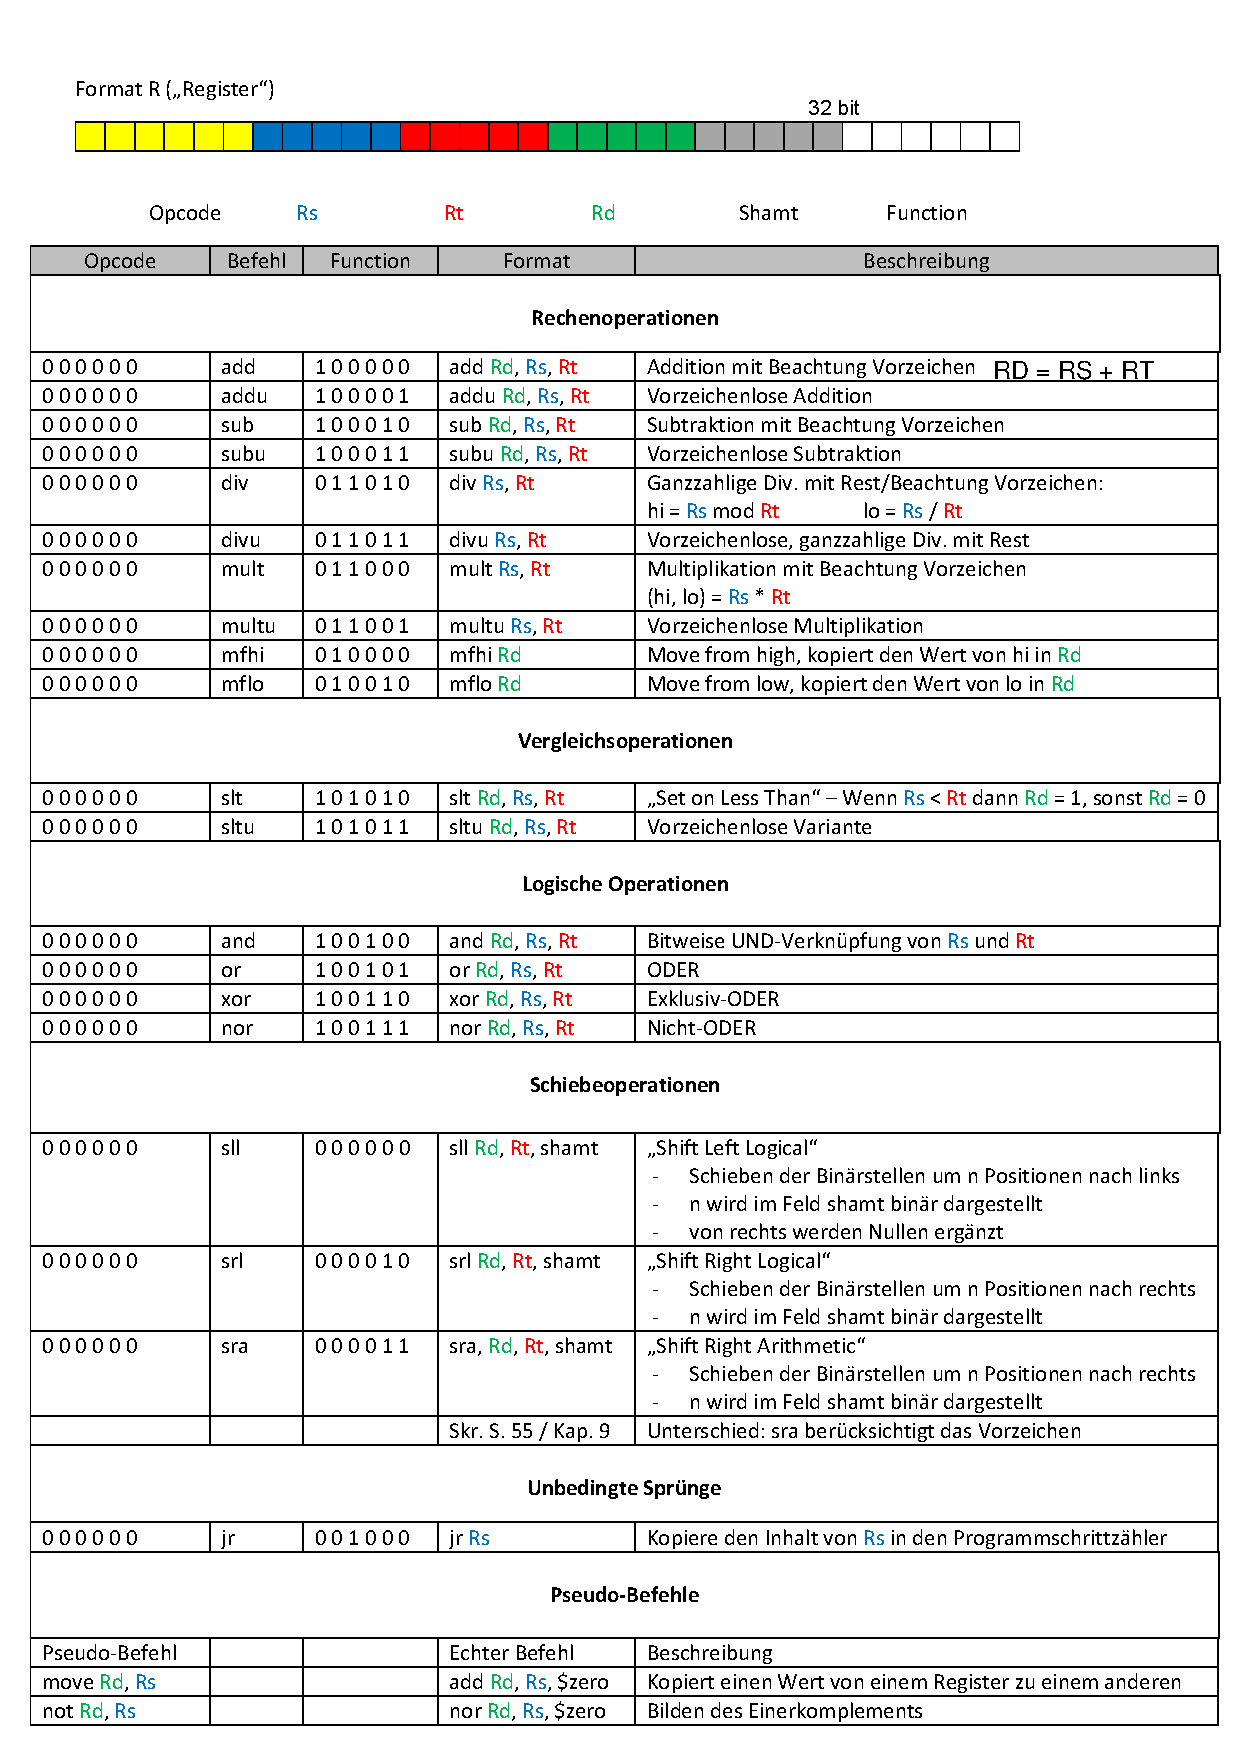
\includepdf[pages={1,2,3}]{Uebersicht_Assemblerbefehle.pdf}
\end{document}


